\section{Q\&A , Examples and Hints}\label{qa-examples-and-hints}

\textbf{Example of MandelboxMenger UI}

Example settings

(copy to clipboard, then load in Mandelbulber using : File -- Load settings from
clipboard):

\# Mandelbulber settings file

\# version 2.08

\# only modified parameters

{[}main\_parameters{]}

ambient\_occlusion\_enabled true;

camera 1.872135433718922 -2.023030528885091 1.871963531652841;

camera\_distance\_to\_target 0.005814178381115117;

camera\_rotation -28.76425655707408 26.3550335393397 3.450283685696816;

camera\_top -0.1604796308669786 -0.4174088010201082 0.894436236356597;

DE\_factor 0.6;

dont\_add\_c\_constant\_1 true;

flight\_last\_to\_render 0;

formula\_1 91;

formula\_2 61;

formula\_iterations\_2 5;

formula\_start\_iteration\_2 4;

formula\_stop\_iteration\_2 5;

fractal\_constant\_factor 0.9 0.9 0.9;

fractal\_enable\_2 false;

fractal\_rotation 0 -90 0;

keyframe\_last\_to\_render 0;

main\_light\_beta 44.34;

main\_light\_intensity 2;

mat1\_coloring\_palette\_offset 12.83;

mat1\_coloring\_palette\_size 255;

mat1\_surface\_color\_palette fd6029 698403 fff59c 000000 0b5e87 c68876 a51c64
3b9fee d4ffd4 aba53c;

SSAO\_random\_mode true;

target 1.874642452030676 -2.018463533070165 1.874544631933419;

view\_distance\_max 28.58330790625501;

volumetric\_fog\_colour\_1\_distance 3.55841069795292e-06;

volumetric\_fog\_colour\_2\_distance 7.116821395905841e-06;

volumetric\_fog\_distance\_factor 7.116821395905841e-06;

{[}fractal\_1{]}

fold\_color\_comp\_fold 0.3;

mandelbox\_color -0.27 0.05 0.07000000000000001;

mandelbox\_rotation\_main 9 1.74 3;

mandelbox\_scale -1.5;

transf\_addCpixel\_enabled\_false true;

transf\_int\_1 12;

transf\_scaleB\_1 0;

transf\_scaleC\_1 0;

transf\_start\_iterations\_M 4;

transf\_stop\_iterations\_M 5;\\[2\baselineskip]1) In the example the
MengerSponge part is run only on iteration 4. A single iteration of another
fractal to make a hybrid is often the best practice.\\[2\baselineskip]2) In the
Statistics (enable in View menu) you can see Percentage of Wrong Distance
Estimations ("Bad DE") is 0, which is good!!. As a general rule less than 0.01
is good, but it is case specific and 3.0 sometimes is OK and .0001 sometimes is
not.

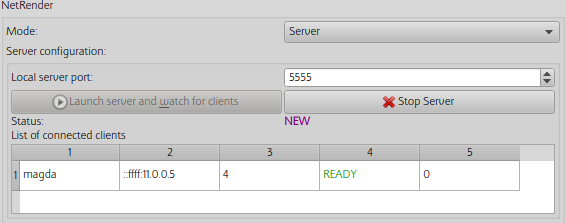
\includegraphics[width=4.51024in,height=2.48976in]{img/manual/media/image31.png}\\[2\baselineskip]T

The Raymarching step multiplier or "fudge factor" (Rendering Engine tab) is set
at 0.6, which is good for a hybrid. If I change it to 0.7 the Percentage of Bad
DE leaps up to 0.25 and you can see the areas of quality loss on your
image.\\[2\baselineskip]Now if we disable the addCpixel Axis swap Constant
Multiplier, we find we can now increase the Raymarching Step Multiplier to 0.9,
and get a faster render and visually the same quality. So monitoring Percentage
of Wrong Distance Estimations is a guide to managing quality. ( Note when doing
animations you may want to drop the Raymarching step down a bit to allow for
what might happen between keyframes.)\\[2\baselineskip]3) MandelboxMenger
Hybrids can behave a bit differently to a lot of hybrids, in the fact that the
Percentage Bad DE often improves when you zoom in.

\textbf{maximum view distance}

Located : Rendering Engine - Common Rendering settings\\[2\baselineskip]It is
important to optimize this setting to minimize render time. You can reduce until
the furthest part of the 3D object(s) starts to disappear. However with
animation an allowance should be made for changes between
keyframes.\\[2\baselineskip]hint/note.\\ When navigating in Relative step mode,
mouse click on spherical\_inversion, camera zooms out, tand maximum view
distance becomes set on 280. If you don't reset it your render times will be
increased.

\textbf{Magic Angle} Benesi Mag Transforms

In mathematics the Magic Angle = 54.7356° .

When rendering basic mag transforms the image does not render parallel to the
standard x,y,z global axis. On the fractal dock, in ``Global parameters'' set
y-axis rotation to 35.2644° ( = 90° - 54.7356°). The fractal will then render
parallel to the x-y plane.

\textbf{Example of using Transform\_Menger Fold to make
	Hybrid}\\[2\baselineskip]\# Mandelbulber settings file

\# version 2.08

\# only modified parameters

{[}main\_parameters{]}

ambient\_occlusion\_enabled true;

camera -1.528388569045064 -1.23063017895654 -0.0251755516595821;

camera\_distance\_to\_target 0.0004503351519815117;

camera\_rotation -14.07789975269277 -44.28785609194563 3.773777260910995;

camera\_top 0.2333184436621841 0.6598138513697914 0.7142885869084139;

DE\_factor 0.7;

flight\_last\_to\_render 0;

formula\_1 1052;

formula\_2 1010;

formula\_3 1052;

formula\_4 1009;

formula\_iterations\_1 5;

formula\_start\_iteration\_4 45;

formula\_stop\_iteration\_2 12;

formula\_stop\_iteration\_4 5;

fractal\_constant\_factor 0.9 0.9 0.9;

fractal\_enable\_4 false;

hdr true;

hybrid\_fractal\_enable true;

keyframe\_last\_to\_render 0;

main\_light\_alpha 2.6;

main\_light\_beta 1.59;

mat1\_coloring\_palette\_offset 46.51;

mat1\_coloring\_palette\_size 255;

mat1\_coloring\_random\_seed 647723;

SSAO\_random\_mode true;

target -1.528310155903731 -1.230317492741513 -0.02549000429402527;

volumetric\_fog\_colour\_1\_distance 3.55841069795292e-06;

volumetric\_fog\_colour\_2\_distance 7.116821395905841e-06;

volumetric\_fog\_distance\_factor 7.116821395905841e-06;

{[}fractal\_1{]}

transf\_addition\_constantA\_000 -0.071633 0 0;

transf\_function\_enabledy false;

transf\_int\_1 12;

transf\_scale 0.5;

transf\_scaleC\_1 0;

transf\_stop\_iterations\_1 2;

{[}fractal\_2{]}

transf\_scale3D\_333 1.055556 1.027778 0.861111;

{[}fractal\_3{]}

transf\_function\_enabledx false;

On this transform UI, the standard menger sponge formula is split into a start
and end function. The simplest way to use this transform is in Hybrid Mode,
having the menger fold transform in slots 1 \& 3. In slot 2 place any linear
type formula or transform. (ie more mengers, kifs, mboxes, amazing surf, folds,
rotation , Benesi T1 etc).\\[2\baselineskip]In slot 1 disable the stop function
and in slot 3 disable the start function, resulting in a standard menger sponge
with something in the middle.\\[2\baselineskip]BTW in fact you can mix around
with the start and stop functions have all enabled if you wish. Generally linear
functions all work well together in making hybrids.\\[2\baselineskip]In
Statistics, maximum is approx. 80 iterations. Generally hybrids take longer to
render than standard formulas.\\ As well as adjusting formula parameters, you
can use the iteration controls to tweak hybrids. In this example the first slot
is set to repeat for 5 iterations before moving to slot 2. Slot 2 is set to stop
at iteration 12, whereas slots 1 \& 3 can continue to termination conditions are
met (bailout or maximum number of iterations).

In the example above, slot2 of the hybrid sequenced ended at iteration 12. 12
was chosen because how it fitted into the iteration sequence, as follows:\\
Slot1 x 5\\ 0,1,2,3,4~ iteration numbers (note first iteration is iteration
number 0.)\\ slot2\\ 5\\ slot3~\\ 6\\ slot1 x 5\\ 7,8,9,10.11\\ slot2\\ 12~ //
last use of slot2\\ \hspace*{0.333em}sequence continues slot1 x 5, slot3,
.....to bailout.\\ So slot2 is used only twice in the iteration process. If I
had entered 11 instead of 12 for slot2's stop\_iterations, then the slot would
have been used only once, if I entered 19 then it would run three times.

\subsection{Q\&A . How do you get different materials on different
	shapes?}\label{qa-.-how-do-you-get-different-materials-on-different-shapes}

This is how I have been doing it.\\[2\baselineskip]\emph{Rectangle at the bottom
	marked A.}\\[2\baselineskip]This is where you~ start a new material or load an
existing.~ The active material is highlighted in blue. Meaning it is active in
the \textbf{material editor} where you create or modify the
material.\\[2\baselineskip]\emph{Rectangle at top left marked
	B.}\\[2\baselineskip]One way to use a material is to go to Global Parameters,
click on the material preview image, and the \textbf{Material Manager} UI will
appear with the materials you have loaded or created. Click on the one you want
to use, then close that UI.\\ Similarly with primitives, click on the material
preview image. And with Boolean Mode each fractal/transform has it's own
material preview image when you scroll down.

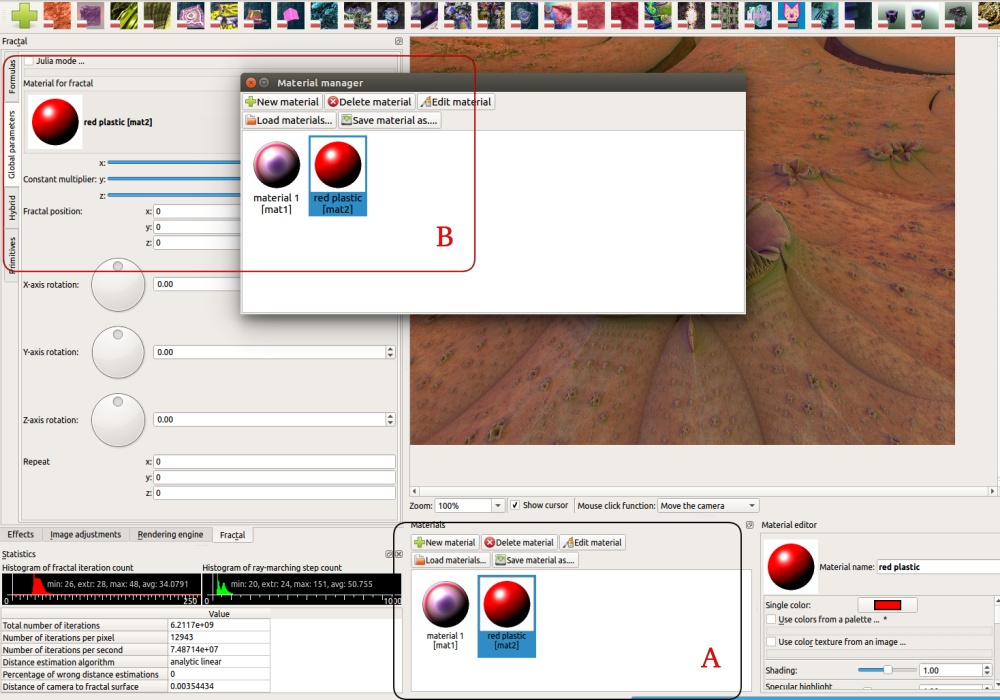
\includegraphics[width=6.69291in,height=4.68465in]{img/manual/media/image32.jpg}

